\section{Antennas}

The primary objective is to establish a reliable telemetry and command link between the rocket and the Ground Control Station (GCS). The system must support real-time telemetry downlink and command uplink throughout the mission profile, from launch to apogee and subsequent descent.  

The 433 MHz band offers a superior propagation profile compared to 2.4 GHz, significantly reducing free-space path loss (FSPL). This lower frequency improves signal penetration through potential ground obstacles and atmospheric phenomena, which is critical for maintaining link margin at long ranges with low transmitter power. 

The primary justification for selecting 433 MHz is the minimization of FSPL. The theoretical signal loss at apogee (3.2 km) is calculated using the Friis Transmission Equation in logarithmic form below. Considering d = 3.2 km (Maximum range) and f = 433.15 MHz the loss is approximately 95.2 dB, the 32.44 factor comes from the conversion of distance to km and Hz to MHz. 

The link margin will serves as a measure of reliability, representing the safety buffer between the received signal and the system's sensitivity floor. 

\begin{itemize}
    \item Tx Power (LoRa Ra-02): \(+20 \,\text{dBm}\)
    \item Tx Antenna (Rocket Omni): \(0 \,\text{dBi}\)
    \item Path Loss (at 3.2 km): \(-95.2 \,\text{dB}\)
    \item Rx Antenna (GCS Yagi): \(+9.7 \,\text{dBi}\)
    \item Cable/Connector Losses: \(-2 \,\text{dB}\)
\end{itemize}

The estimated Received Power is $P_{rx}=20-95.2+9.7-2=-67.5\mathrm{\ dBm}$. Given the LoRa SX1278 sensitivity of approximately -130 dBm (at SF12), the final margin is 
Margin = $\mathrm{M\arg in}=P_{rx}-P_{sensitivity}=-67.5-\left(-130\right)=62.5\mathrm{dB}$. A 62.5 $\mathrm{dB}$ margin is highly robust, allowing the system to tolerate significant tumbling (polarization mismatch), Yagi misalignment, or interference while maintaining a signal lock. 

\begin{figure}[ht]
    \centering
    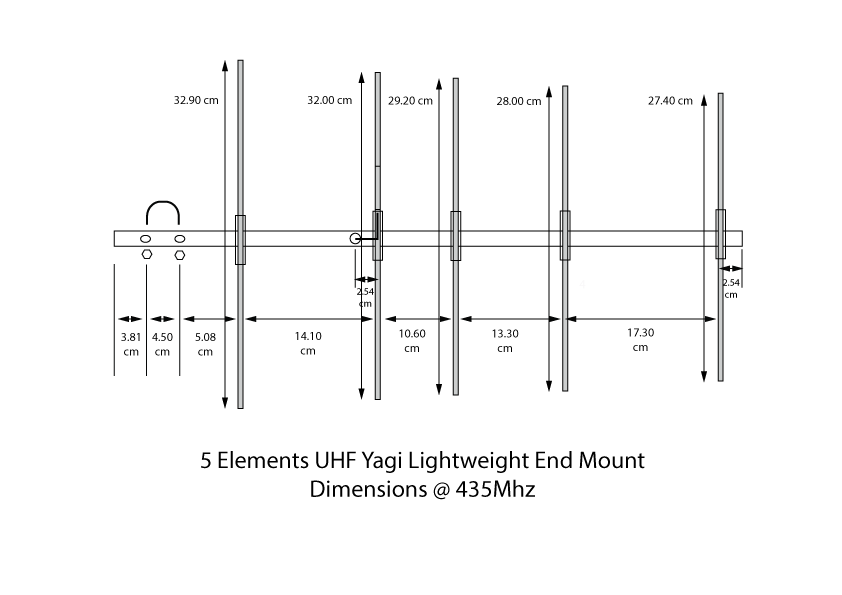
\includegraphics[width=0.85\textwidth]{Images/4_Communication/5_Elements_UHF.png}
    \caption{5-element Yagi-Uda antenna geometry}
    \label{fig:yagi_geometry}
\end{figure}

The physical dimensions of the Yagi elements (Reflector length approx. 329 mm) directly correlate to the 433 MHz band. Using the standard approximation for a half-wave element 
$\lambda=\frac cf \approx \frac{300}{433} \approx 0.693m \Rightarrow \lambda/2 \approx 346mm$. 

The measured element lengths (e.g., Reflector at 329mm) are shorter than the standard free-space half-wave dipole (346 mm) to account for the Boom Correction Factor. Since the boom is made of conductive aluminum, it electrically interacts with the parasitic elements. When an element passes through or connects to a metal boom, the boom acts as a shorted turn, effectively lengthening the element electrically. To compensate for this and maintain resonance at 433.15 MHz, the physical elements must be shortened. For a 20 mm boom, elements are typically reduced by 15-20 mm compared to a non-conductive boom: 

$\lambda/2 = 346\mathrm{mm} - 17\mathrm{mm} \approx 329\mathrm{mm}$ 

The choice of a Gamma Match feed is also dictated by the conductive aluminum boom. In this design, the center of the driven element is electrically grounded to the boom. This creates a strong mechanical bond and eliminates static charge buildup. A standard Yagi driven element has a low natural impedance (20 $\Omega$). The Gamma match transforms this low impedance up to the 50 $\Omega$ required by the coaxial cable and transceiver. The slider mechanism on the Gamma match allows for precise VSWR tuning at 433.15 MHz, compensating for any environmental detuning at the launch site. 

The electromagnetic performance of the 5-element Yagi-Uda array was analyzed using  MATLAB's Antenna Toolbox. The simulation model uses the exact physical dimensions defined in the hardware design.  

\begin{figure}[ht]
    \centering
    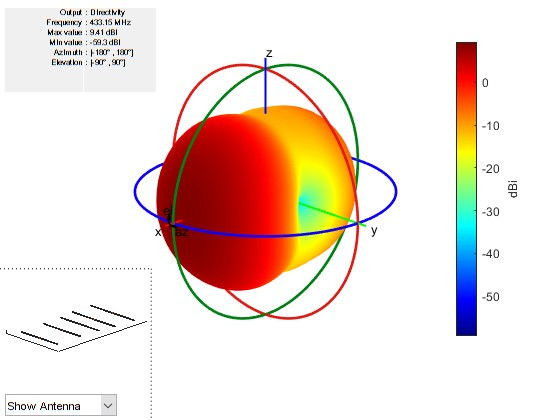
\includegraphics[width=0.85\textwidth]{Images/4_Communication/Simulated_3D_Radiation_Pattern.png}
    \caption{Simulated 3D radiation pattern of the 5-element Yagi-Uda array}
    \label{fig:3d_pattern}
\end{figure}

Distinct from the real antenna, this simulation models a direct split-feed dipole excitation rather than the Gamma Match mechanism or the conductive boom. Consequently, the simulation results present the resonance of the shortened elements (approximately 440 MHz) prior to the inductive correction provided by the Gamma Match.

The simulated 3D radiation pattern shown in Figure \ref{fig:3d_pattern} confirms that the parasitic arrangement successfully focuses RF energy into a single dominant forward lobe. The analysis yields a maximum directivity of 9.41 dBi, which provides a signal amplification of approximately 8.7 times compared to an isotropic radiator. The beam is strictly aligned with the boom axis (Azimuth $0^\circ$, Elevation $0^\circ$), validating the element spacing and phasing.

\begin{figure}[ht]
    \centering

    \begin{subfigure}{0.48\textwidth}
        \centering
        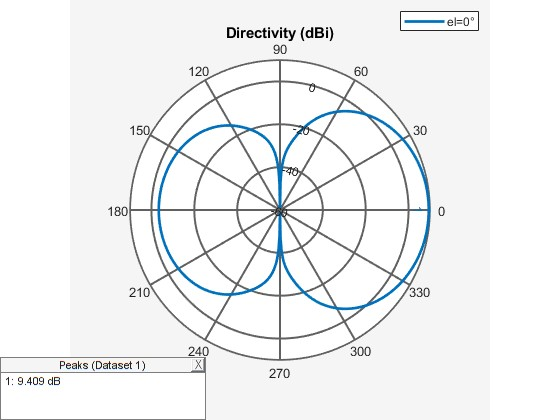
\includegraphics[width=\linewidth]{Images/4_Communication/E_Plane_horizontal_cut.png}
        \caption{E-plane horizontal cut}
        \label{fig:e_plane}
    \end{subfigure}
    \hfill
    \begin{subfigure}{0.48\textwidth}
        \centering
        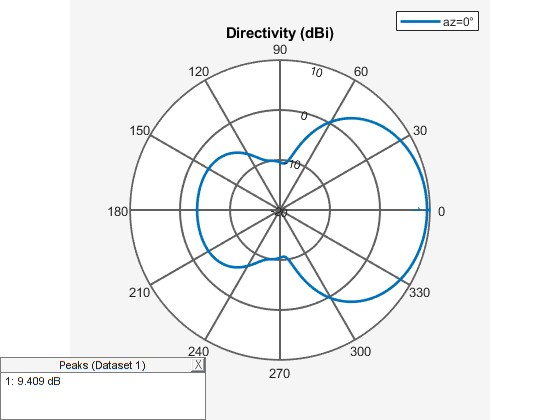
\includegraphics[width=\linewidth]{Images/4_Communication/H-Plane_vertical_cut.png}
        \caption{H-plane vertical cut}
        \label{fig:h_plane}
    \end{subfigure}

    \caption{Radiation pattern plane cuts}
    \label{fig:plane_cuts}
\end{figure}

To define the operational requirements for the Ground Station, we analyze the 2D pattern cuts. The vertical cut shown in Figure \ref{fig:h_plane} displays the pattern perpendicular to the elements. The main beam is broad, offering a Half-Power Beamwidth (HPBW) of approximately 60º. The horizontal cut shown in Figure \ref{fig:e_plane} displays the pattern parallel to the elements. The pattern exhibits deep nulls at 90º, which aids in rejecting interference from lateral sources. 

\begin{figure}[ht]
    \centering
    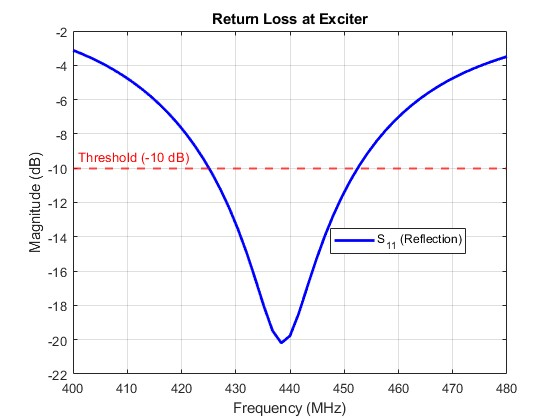
\includegraphics[width=0.85\textwidth]{Images/4_Communication/return_loss.png}
    \caption{Simulated return loss ($S_{11}$) of the antenna}
    \label{fig:return_loss}
\end{figure}

The broad HPBW implies that the ground station operator has a generous tracking window. The antenna can be misaligned by up to 30º from the rocket's position while still maintaining a signal strength within 3 dB of the peak. This eliminates the need for high-precision automated tracking systems. 

A critical aspect of this design is the interaction between the physical element lengths and the feed mechanism. Figure \ref{fig:return_loss} shows the return loss ($S_{11}$) of the simulated structure.

The simulation shows the resonance dip centered at approximately 440 MHz, rather than the target 433.15 MHz. This is an expected result because of the boom correction effect and the gamma match feed role. 

The physical elements were intentionally shortened (e.g., Reflector 329mm instead of the theoretical 346mm) to compensate for the conductive aluminum boom, which electrically lengthens elements in the real world. Since the MATLAB simulation models free-space elements (no boom), it accurately reports that these short elements resonate at a higher frequency (440 MHz). 

In the physical assembly, the Gamma Match provides the necessary inductance to lower the resonant frequency from 440 MHz to 433.15 MHz, while simultaneously transforming the feed impedance to 50$\Omega$. 

This simulation confirms that the physical dimensions are correct for a boom-mounted, Gamma-matched implementation. If the simulation had shown resonance at 433 MHz using these short lengths without the boom model, the physical antenna would likely have been tuned too low (e.g., 420 MHz) once built. 

The analysis confirms that the 5-element Yagi provides the necessary 9.4 dBi gain to close the link budget at the 3.2 km apogee. The combination of high forward gain and a manageable 60º beamwidth satisfies the mission requirement for a reliable, manually trackable uplink/downlink. 